\chapter{Overview}
\ac{ESSIG} is roughly composed out of three components. There is a generator,
an interpreter and a debugger frontend. The generator reads in a specification
of the microcontroller %(see \autoref{Microcontroller specification language})
and generates code that will simulate the instructions. It also generates code
that describes an opcode table and some other attributes of microcontroller.
The interpreter or Virtual Machine (VM) interfaces with the generated code, and
basically does all the work of allocating memory for the simulation,
disassembling the instructions and calling the right opcode handlers. These two
components will hereafter be referred to as the Simulator. Lastly there is the
debugger frontend, which links with the Simulator and provides a command line
debugger interface for the user to control the simulation process.

\begin{comment}
First we have
the input language, which can be used to describe the micro controller a
simulator should be generated for. Than we have a generator, which
creates an implementation of the private API (see VM) that the VM can
use in simulating the micro controller. Than we have our VM, in which
the micro controller will be simulated. It exposes a public API to a
client which can then simulate programs like they were running on the
simulator. The following diagram illustrates how the components relate
to each other.
\end{comment}


\begin{center}
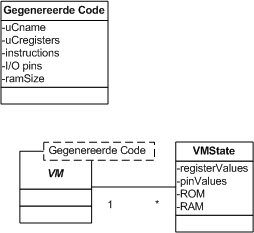
\includegraphics{diagrams/Model.png}
\end{center}
